\begin{figure}
	\begin{subfigure}{\linewidth}
	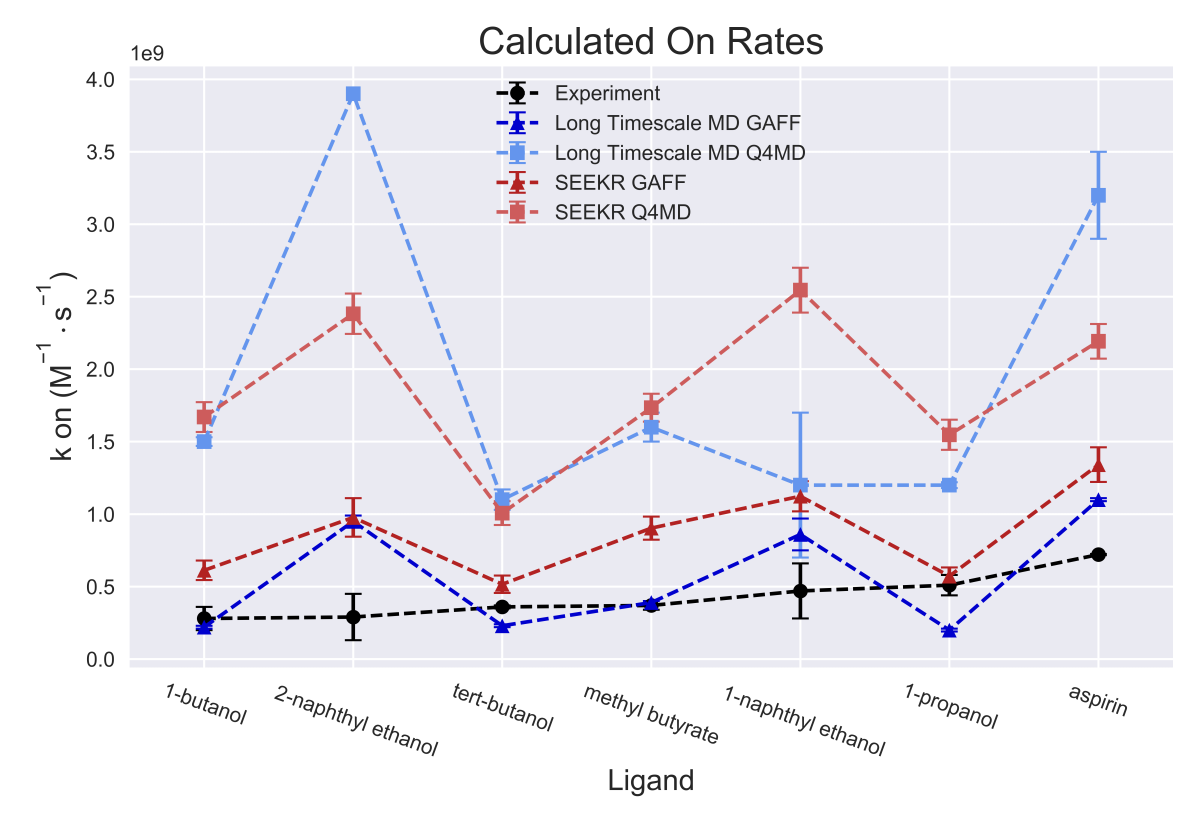
\includegraphics{images/on_scatter_resize.png}
	\caption{}
	\end{subfigure}

	\bigskip
	

	\begin{subfigure}{\linewidth}%<-- changed width
		%\centering
        %\renewcommand\tabularxcolumn[1]{m{#1}}% <-- added
        %\renewcommand\arraystretch{1.3}
        %\setlength\tabcolsep{2pt}% <-- added
    \begin{tabular}{
l  S[table-format = 2.3(3), separate-uncertainty] 
  S[table-format = 2.3(3), separate-uncertainty] 
 }%{\linewidth}%{*{4}{>{\centering\arraybackslash}X}}% <-- changed

\textbf{Method} & \textbf{Kendall} & \textbf{Spearman}  \\
\hline
      SEEKR GAFF      &    -0.20(31)           &    -0.29(40)            \\ 
      SEEKR Q4MD      &    0.14(29)           &    0.14(38)             \\ 
      Long Timescale MD GAFF      &    0.24(26)           &    0.25(29)                     \\ 
      Long Timescale MD Q4MD      &    0.00(28)           &    -0.05(37)                     \\ 
     

    \end{tabular}
        \caption{}
	\end{subfigure}
	\caption{a) Experimental and calculated on rates for SEEKR GAFF and Q4MD forcefields as well as long timescale MD with both forcefields. b) Calculated rank correlation coefficients. Errors are determined with a bootstrapping analysis. }
  \label{fig:on_scatter}
  \end{figure}